\begin{center}
    {\LARGE \textbf{2022有机化学与分析化学}} \\[2ex]
    {\large 时量180分钟 \quad 满分150分}
\end{center}

\vspace{0.5cm}
\noindent\textbf{注意事项:}
\begin{enumerate}[label=\arabic*., parsep=0pt, itemsep=0pt]
    \item 答题前,考生先将自己的姓名、学号、考场号、座位号填写在答题卡上,将条形码准确粘贴在考生信息条形码粘贴区。
    \item 考试结束后,将本试卷与答题纸一并收回。
    \item 回答各个问题时,将答案写在答题纸上,写在本试卷上无效。
\end{enumerate}

\vspace{1cm}
\begin{center}
    {\Large \textbf{有机化学部分(共100分)}}
\end{center}

\vspace{0.5cm}
\noindent\textbf{一、选择题（15 pts.）}

\begin{enumerate}[label=\arabic*., itemsep=1.5ex]
    \item 下列碳正离子中，最稳定的是
    
    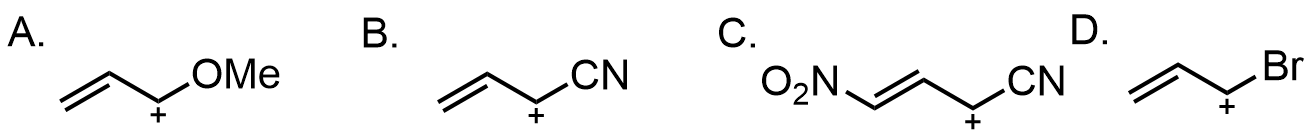
\includegraphics[scale=0.38, valign=c]{./Figure/2022/2022_4_1.png}
    \item 不能与饱和亚硫酸氢钠溶液反应的化合物是
    \begin{tasks}(4)
        \task 环戊酮
        \task 葡萄糖
        \task 苯甲醛
        \task 2-丁酮
    \end{tasks}
    \item 不能发生碘仿反应的化合物是
    \begin{tasks}(4)
        \task 苯乙酮
        \task 乙醇
        \task 乙醚
        \task 乙酰乙酸乙酯
    \end{tasks}
    \item 下列化合物中，酸性最强的是
    
    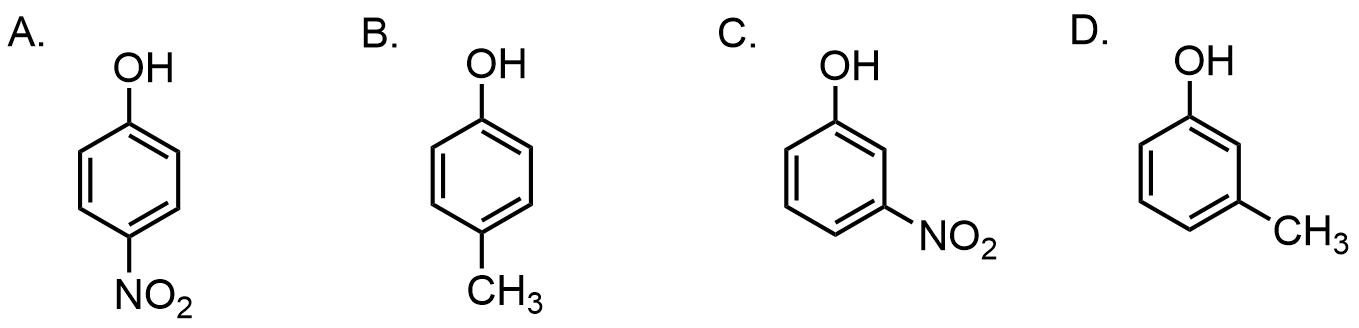
\includegraphics[scale=0.38, valign=c]{./Figure/2022/2022_4_4.png} 
    \item 下列化合物中，不具有芳香性的是
    
    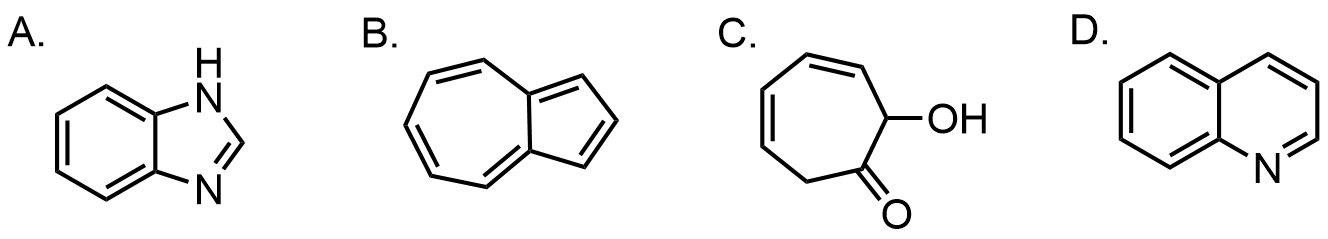
\includegraphics[scale=0.38, valign=c]{./Figure/2022/2022_4_5.png}
    \item 下列化合物中，具有手性的分子是
    
    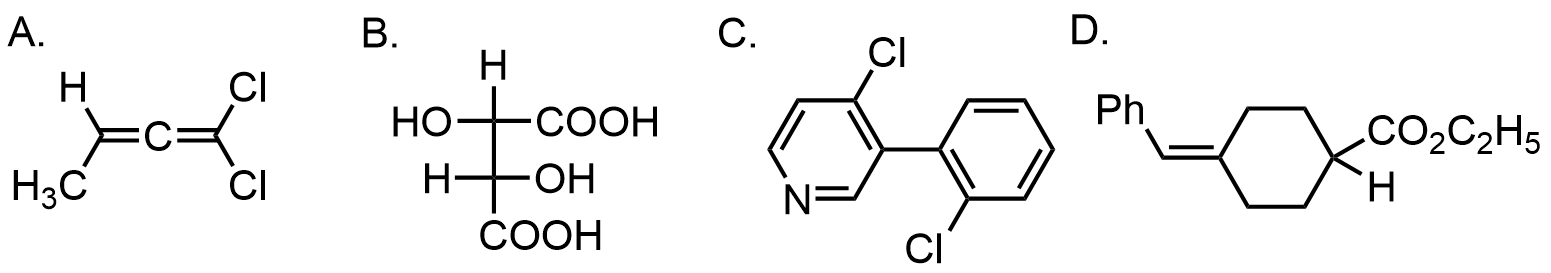
\includegraphics[scale=0.38, valign=c]{./Figure/2022/2022_4_6.png}
    \item 下列化合物中，碱性最强的是
    
    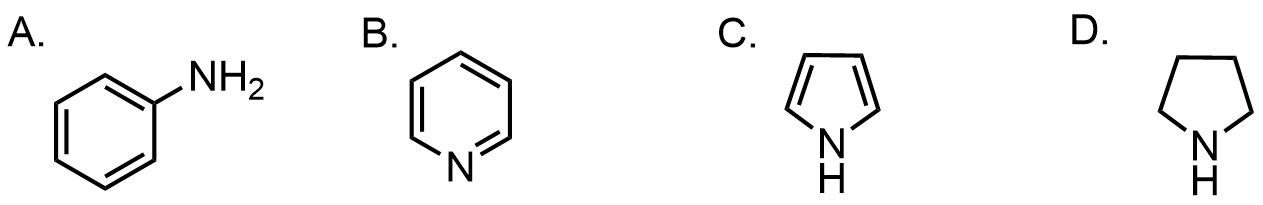
\includegraphics[scale=0.38, valign=c]{./Figure/2022/2022_4_7.png} 
    \item 下列化合物构象最稳定的是
    
    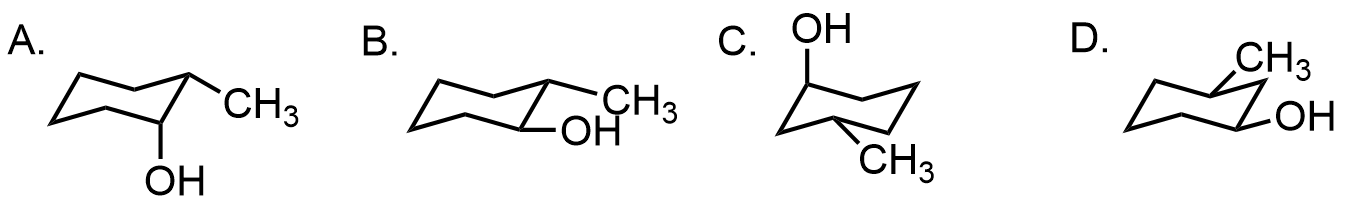
\includegraphics[scale=0.38, valign=c]{./Figure/2022/2022_4_8.png} 
    \item 下列亲双烯体中，[4+2]环加成反应活性最高的是
    
    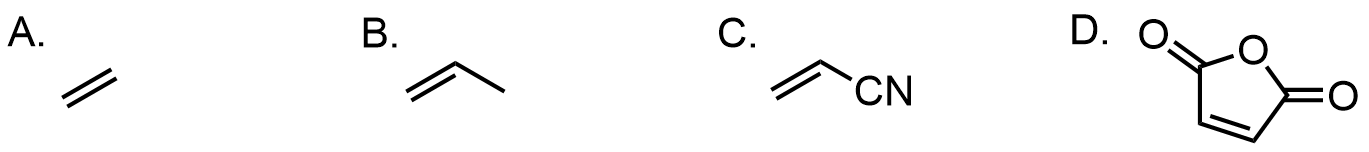
\includegraphics[scale=0.38, valign=c]{./Figure/2022/2022_4_9.png}
    \item 下列化合物中，不能被稀酸水解的是
    
    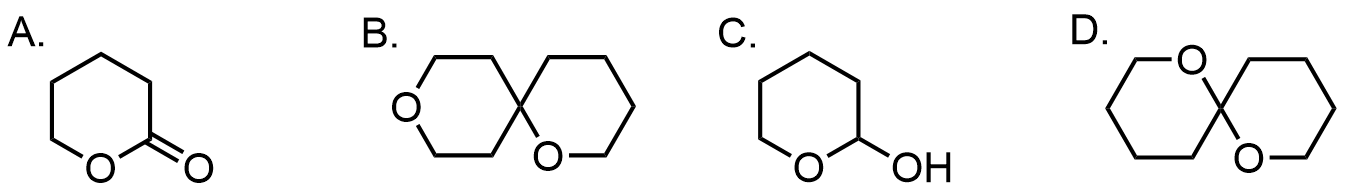
\includegraphics[scale=0.38, valign=c]{./Figure/2022/2022_4_10.png}
    \item 在四氯化碳中，下列化合物烯醇式含量最高的是
    
    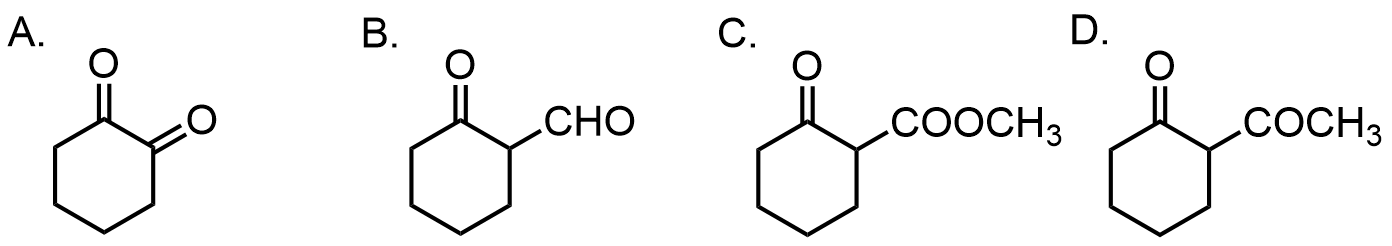
\includegraphics[scale=0.38, valign=c]{./Figure/2022/2022_4_11.png}
    \item 下列试剂不能把羰基还原为亚甲基的是
    \begin{tasks}(2)
        \task Zn(Hg),HCl
        \task KOH/\ce{O(CH2CH2OH)2}/\ce{NH2NH2}
        \task \ce{LiAlH4}
        \task \ce{HSCH2CH2SH}/\ce{Pt}
    \end{tasks}
    \item 下列试剂中，亲核性最好的是
    \begin{tasks}(2)
        \task \ce{CH3CH2COO-}
        \task \ce{CH3CH2S-}
        \task \ce{CH3CH2O-}
        \task \ce{CH3CH2SH}
    \end{tasks}
    \item 下列羰基化合物与\ce{CH3MgI}反应时，慢反应一步活化能最低的是
    
    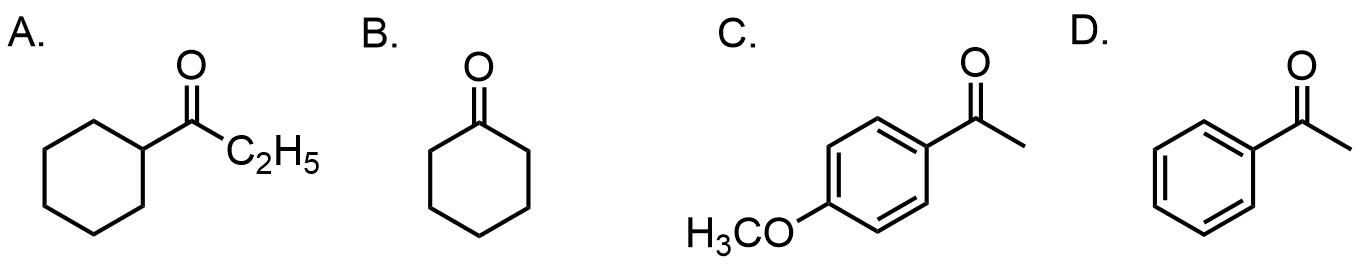
\includegraphics[scale=0.38, valign=c]{./Figure/2022/2022_4_14.png}
    \item 下列共振式中对杂化体贡献最大的是
    
    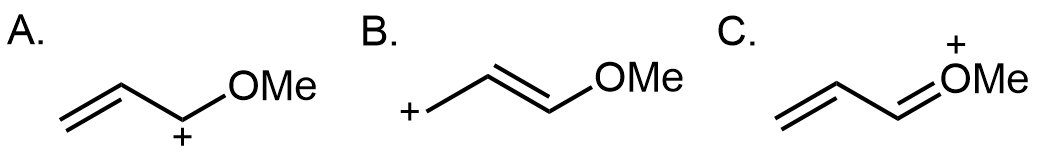
\includegraphics[scale=0.38, valign=c]{./Figure/2022/2022_4_15.png}

\end{enumerate}

\vspace{0.5cm}
\noindent\textbf{二、完成反应(30 pts.)}

\begin{enumerate}[label=\arabic*., itemsep=3ex]
    \item 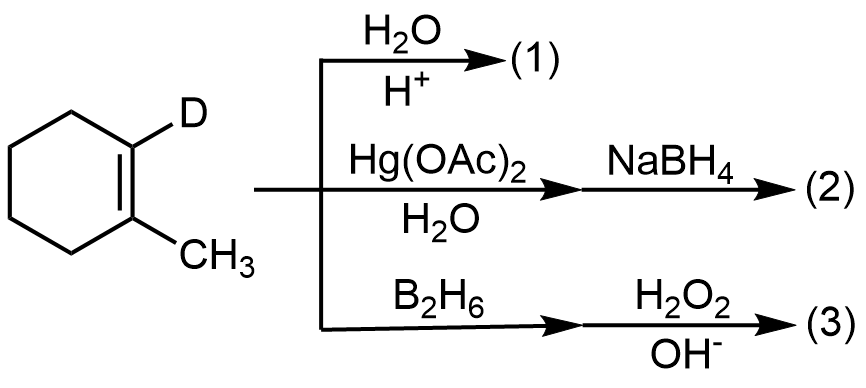
\includegraphics[scale=0.3, valign=c]{./Figure/2022/2022_1_1.png} 
    \item 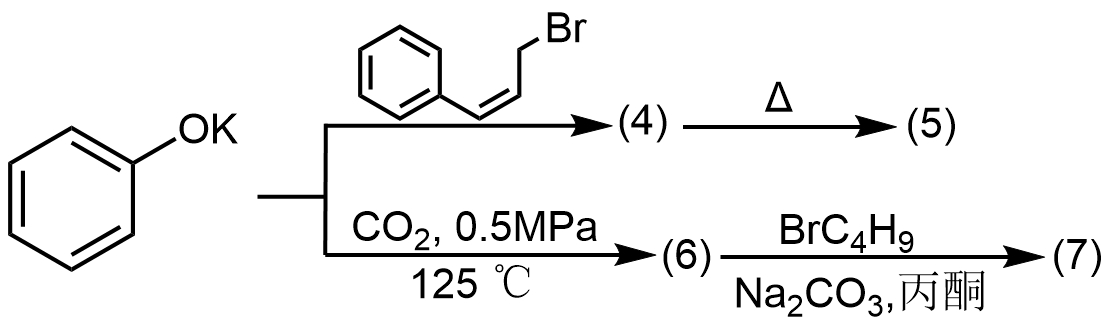
\includegraphics[scale=0.3, valign=c]{./Figure/2022/2022_1_2.png}
    \item 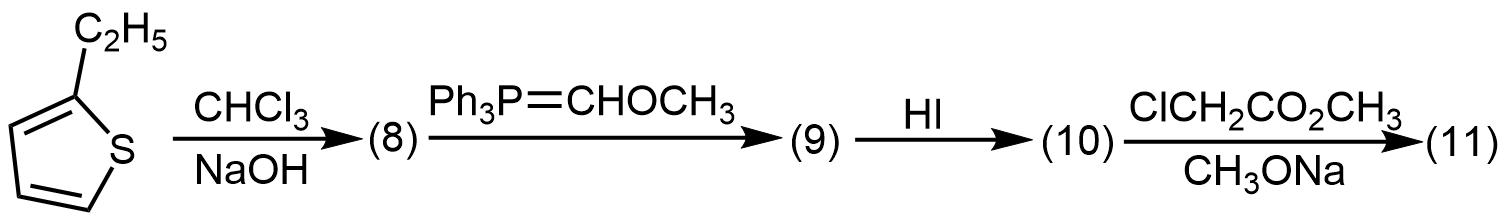
\includegraphics[scale=0.3, valign=c]{./Figure/2022/2022_1_3.png}
    \item 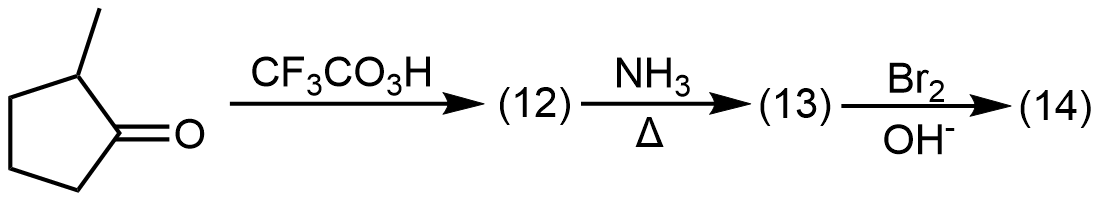
\includegraphics[scale=0.3, valign=c]{./Figure/2022/2022_1_4.png}
    \item 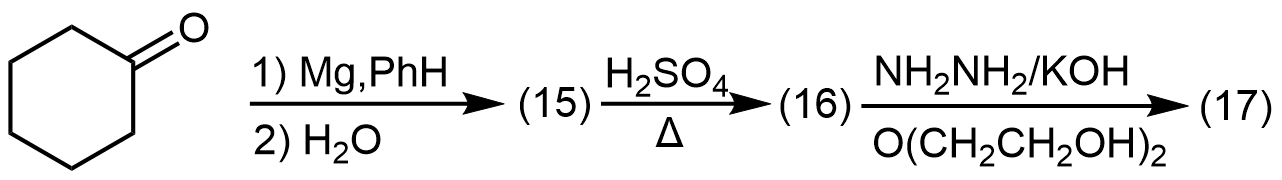
\includegraphics[scale=0.3, valign=c]{./Figure/2022/2022_1_5.png}
    \item 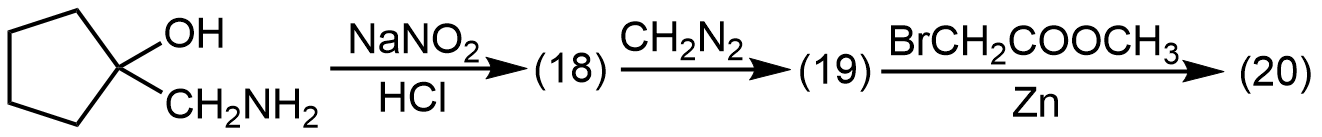
\includegraphics[scale=0.3, valign=c]{./Figure/2022/2022_1_6.png}
    \item 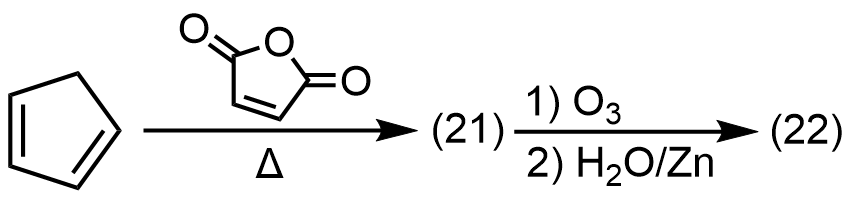
\includegraphics[scale=0.3, valign=c]{./Figure/2022/2022_1_7.png}
    \item 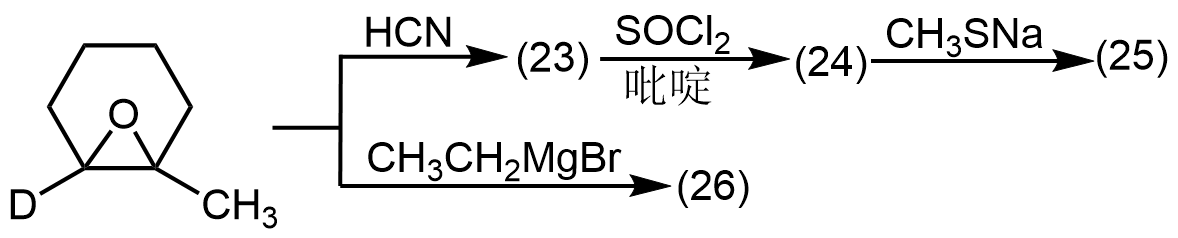
\includegraphics[scale=0.3, valign=c]{./Figure/2022/2022_1_8.png}
    \item 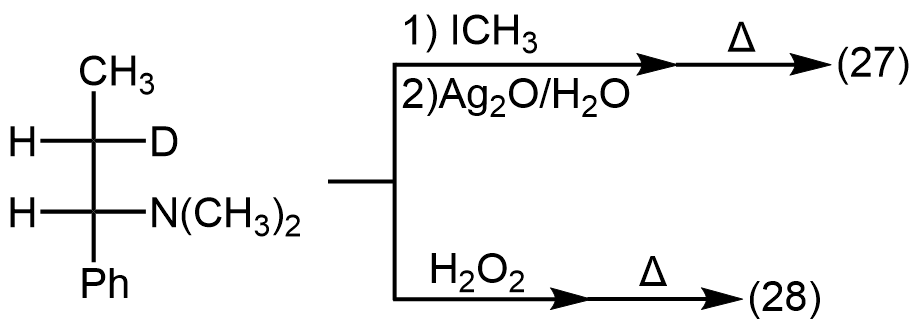
\includegraphics[scale=0.3, valign=c]{./Figure/2022/2022_1_9.png}
    \item 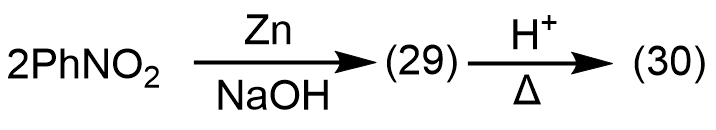
\includegraphics[scale=0.3, valign=c]{./Figure/2022/2022_1_10.png}

\end{enumerate}

\vspace{0.5cm}
\noindent\textbf{三、简答题(6 pts.)}

\begin{enumerate}[label=\arabic*., itemsep=3ex]
    \item 有人想用化合物A通过硝酸硝化得到化合物B，但是却得到了化合物C为主的产物。试解释这一现象。
    
    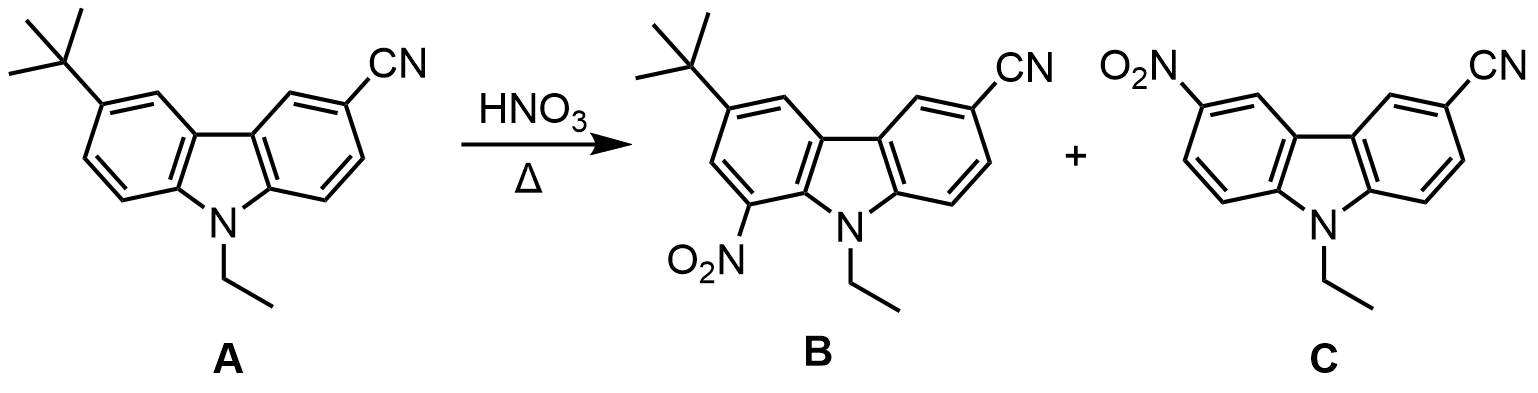
\includegraphics[scale=0.35, valign=c]{./Figure/2022/2022_5_1.png}
\end{enumerate}


\vspace{0.5cm}
\noindent\textbf{四、机理题(14 pts.)}

\begin{enumerate}[label=\arabic*., start=1, itemsep=1.5ex]
    \item 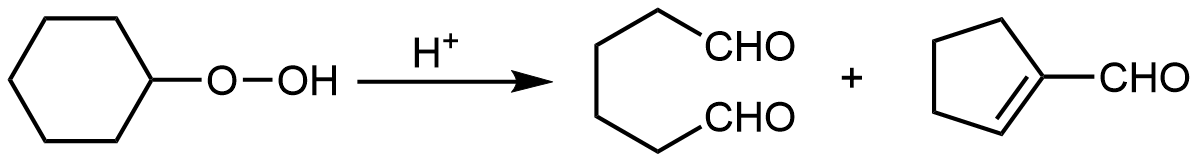
\includegraphics[scale=0.3, valign=c]{./Figure/2022/2022_2_1.png}
    \item 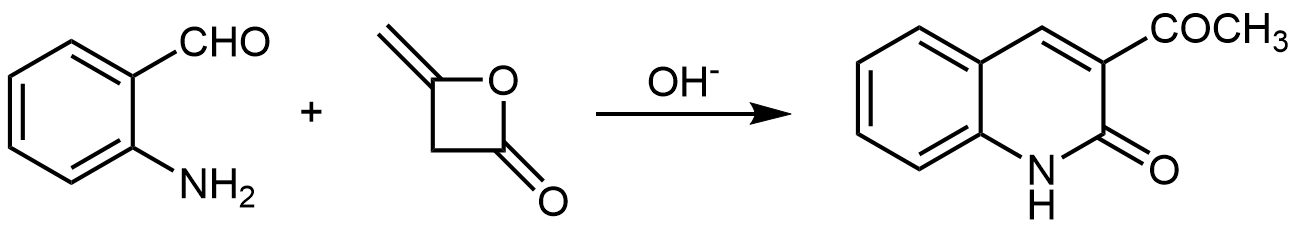
\includegraphics[scale=0.3, valign=c]{./Figure/2022/2022_2_2.png}

\end{enumerate}

\vspace{0.5cm}
\noindent\textbf{五、合成题(35 pts.)}

\begin{enumerate}[label=\arabic*., start=1, itemsep=1.5ex]
    \item 以乙炔为唯一有机原料合成\textbf{A}
    \item 以苯、小于等于2个碳的有机物合成\textbf{B}
    \item 以苯、小于等于3个碳的有机物合成\textbf{C}
    \item 以环己酮、小于等于3个碳的有机物合成\textbf{D}
    \item 以苯、小于等于3个碳的有机物合成\textbf{E}
    
    \begin{center}
        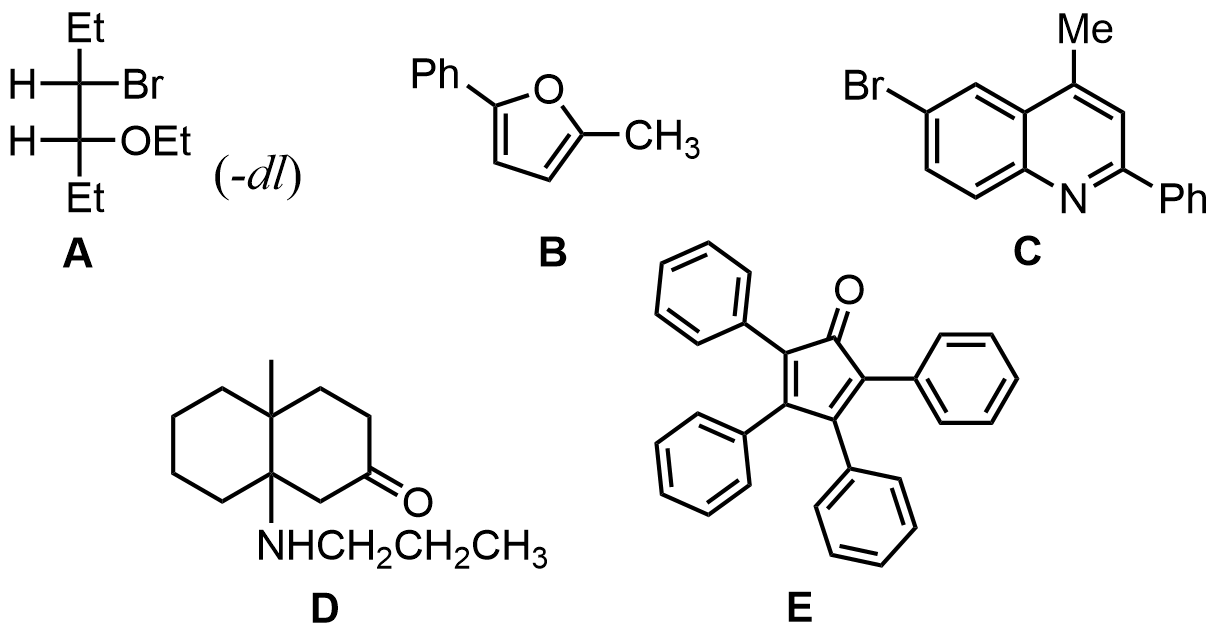
\includegraphics[scale=0.38]{./Figure/2022/2022_3.png}
    \end{center}
\end{enumerate}

\vspace{1cm}
\begin{center}
    {\Large \textbf{分析化学部分(共50分)}}
\end{center}


\vspace{0.5cm}
\noindent\textbf{六、简答题（每小题4分）}

\begin{enumerate}[label=\arabic*., itemsep=1.5ex]
    \item 络合滴定中为什么要加入缓冲溶液?请说明原因。
    \item 写出下列水溶液的质子平衡条件式
    \begin{enumerate}[label=(\arabic*), noitemsep, topsep=0pt, partopsep=0pt]
        \item $(\ce{NH4})_2\ce{CO3}$
        \item $0.2\ \mathrm{mol/L}\ \ce{H2SO4}$
    \end{enumerate}
    \item 简述EDTA的$\lg\alpha_{Y(\mathrm{H})}$随$\mathrm{pH}$的变化趋势，如只考虑酸效应，则金属离子$\ce{M}$与EDTA络合物的条件稳定常数$K'_{\ce{MY}}$的表达式是什么?
    \item 已知半反应$\ce{VO2^+ + 2H^+ + e^- = VO^{2+} + H2O}$的标准电极电位$\varphi^\ominus=1.00\ \mathrm{V}$,计算$\mathrm{pH}=2.00$时，溶液中电对$\ce{VO2^+/VO^{2+}}$的条件电位$\varphi^\ominus{}'$。
    \item 用甲醛法测得某铵盐中氮的质量分数($\%$)为$5.15$, $5.32$, $5.22$, $5.25$,计算含氮量在置信度$95\%$时总体平均值的置信区间。[已知：$t_{0.05,3}=3.18$]
\end{enumerate}

\vspace{0.5cm}
\noindent\textbf{七、计算题（每小题10分，共30分）}

\begin{enumerate}[label=\arabic*., itemsep=1.5ex]
    \item 用$0.1000\ \mathrm{mol/L}\ \ce{NaOH}$溶液滴定$20.00\ \mathrm{mL}\ 0.05000\ \mathrm{mol/L}\ \ce{H2A}$,计算：
    \begin{enumerate}[label=(\arabic*), noitemsep, topsep=0pt, partopsep=0pt]
        \item 化学计量点前$0.1\%$的$\mathrm{pH}$;
        \item 化学计量点的$\mathrm{pH}$;
        \item 化学计量点后$0.1\%$的$\mathrm{pH}$
    \end{enumerate}
    [已知：$\ce{H2A}$的$\mathrm{p}K_{a1}=1.22$,$\mathrm{p}K_{a2}=4.19$]
    \item 以$0.02000\ \mathrm{mol/L}\ \mathrm{EDTA}$滴定浓度均为$0.02000\ \mathrm{mol/L}\ \ce{Zn^{2+}}$、$\ce{Ca^{2+}}$混合液中的$\ce{Zn^{2+}}$,溶液$\mathrm{pH}$为$5.0$,若以二甲酚橙为指示剂，终点误差多大?
    
    [已知：$\mathrm{pH}=5.0$时$\lg\alpha_{Y(\mathrm{H})}=6.6$,$\mathrm{pZn_{ep}}$(二甲酚橙)$=4.8$;$\lg K_{\ce{ZnY}}=16.5$,$\lg K_{\ce{CaY}}=10.7$]
    \item 计算$\ce{AgI}$在$0.01\ \mathrm{mol/L}\ \ce{Na2S2O3}$和$0.01\ \mathrm{mol/L}\ \ce{KI}$混合溶液中的溶解度。
    
    [已知：$\ce{Ag^+}$与$\ce{I^-}$络合$\lg\beta_1\sim\lg\beta_3$依次为$6.58$, $11.74$, $13.68$;$\ce{Ag^+}$与$\ce{S2O3^{2-}}$络合$\lg\beta_1\sim\lg\beta_3$依次为$8.82$, $13.46$, $14.15$; $K_{\mathrm{sp}}(\ce{AgI})=9.3\times10^{-17}$]
\end{enumerate}